\documentclass[10pt]{article}
\usepackage[margin=1in]{geometry}

% use proper unicode fonts
\usepackage[T1]{fontenc}
\usepackage[utf8]{inputenc}

\usepackage{amsmath} % for better display of equations
\usepackage{amssymb}
\usepackage{amsthm}

\usepackage{setspace}
\usepackage[square,sort,comma,numbers]{natbib}
\bibliographystyle{siam}

\onehalfspace

%% Typographic adjustement
\usepackage{microtype}
\usepackage{lipsum}

\usepackage{caption}
\usepackage{subcaption}
\captionsetup{labelfont={bf,small,sf}, textfont={small, sf}}

\setlength{\columnsep}{1cm}

\usepackage{titling} % controls the way the title information is displayed
\pretitle{\begin{flushleft}\Large}
\posttitle{\end{flushleft}}
\predate{}
\postdate{}
\preauthor{\begin{flushleft}}
\postauthor{\end{flushleft}}
\setlength{\droptitle}{-3em}

\setlength{\parskip}{0.5em}

\usepackage{authblk} % adds some nice options for displaying the author list
\renewcommand\Authsep{\protect\\}
\renewcommand\Authands{\protect\\}

%% graphics packages
\usepackage{graphicx}
%\usepackage[nomarkers, tablesfirst]{endfloat} % for final
%\captionsetup{labelsep=none,textformat=empty} % for final
\captionsetup{labelformat=simple} % for drafts
\usepackage{booktabs}
\usepackage[flushleft]{threeparttable}
\usepackage{geometry}

\usepackage{tikz}
\usepackage{pgfplots}
\usepackage{pgfplotstable}
\usepackage{xcolor}
\usetikzlibrary{shapes, arrows, positioning}

%% ----------------------------------
%
%     Title and authorship information
%
%% ----------------------------------


\title{Slow demography constrains the northward expansion of the temperate forest under climate change}

% Title 2
% \title{\textbf{What constrains the northward expansion of the temperate forest?}}

\date{}
\author[1,*]{Steve Vissault (s.vissault@yahoo.fr)}
\author[1,2]{Matthew V. Talluto (mtalluto@gmail.com)}
\author[1]{Isabelle Boulangeat (isabelle.boulangeat@gmail.com)}
\author[1]{Dominique Gravel (dominique\_gravel@uqar.ca)}
\affil[1]{Département de Biologie, Géographie et Chimie, Université du Québec à Rimouski, Rimouski, Québec, Canada}
\affil[2]{Laboratoire d'Écologie Alpine, Université Joseph Fourier, Grenoble, France}
\affil[*]{Author for correspondance. Address: Departement de Biologie, Chimie, et Géographie, 300, Allée des Ursulines, Rimouski, Quebec G5L 3A1, Canada}

\begin{document}

\begin{titlingpage}
		\maketitle

		\begin{flushleft}

			\textbf{Short title:} The future distribution of the northern temperate forest under climate change

			\textbf{Keywords:} states and transitions model, patch occupancy, landscape dynamics, forest inventory databases, community range shift.
		\end{flushleft}
	\end{titlingpage}
	%TC:endignore
	%TC:break abstract


\begin{abstract}
	\noindent
	\textit{\lipsum[1]}
\end{abstract}

\section{Introduction}

Species distribution models (SDMs) are one of the most popular tool to predict impact of climate change on species geographical range \cite{Iverson2002}. Predict forest species range shift under climate change is limited as trees are sessile, long-lived and slow to mature \cite{Lenoir2014a} while SDMs based on correlative methods predict instantaneous vegetation responses; therefore species migration rates are often overestimated using this approach. Integrate ecological processes using process based-model are primordial to improve this prediction \cite{Snell2014a}.  Strong biotic interaction, slow demography and dispersal limitation can conduct to local extinction or prevent species colonization at the leading edge of the species distribution (Source). These ecological mechanisms could limit species spread rate over the forest landscape and could explain why many individual species are failure to migrate \cite{Zhu2012}.

% Paragraphe sur l'implication de mesurer la tension accumuler
Lead unpace with bioclimatic niche
Increase tension
Lead to catastrophic shift with management scenario

% Conclusion: Even if the SDM model provide usefull information such as the species distribution at equilibrium with abiotic condition, the real challenge subsist in predicting if the species will reach this equilibrium and if not what is the main meachnisms limiting his own migration.

% Paragraphe sur l'ecotone Tempérée-Boréal

% Trouver Snell 2011

In this present study, we investigated the range shift and migration rate of the temperate forest at his ecotone using a states and transitions model.   We simulated the ecotone dynamic using different versions of the state and transition model over different climate change scenarios (RCP 8.5, AR5). We compared the models outputs to assess which ecological processes - dispersion,  demography, propagule effect and biotic interaction - are limiting or increasing the migration ability of the temperate forest.



%Justifier le besoin de l'approche par communauté et le besoin d'intégrer processus démographique, dispersion, spatial dynamics

%Multispecies extension of spatial population model


% L'approche par communauté permet de gommer cette variabilité dans la réponses et de d'intéresser davantage aux mécanismes moteurs de la réponses au changements climatiques. Il offre d'augmenter l'intertie du système pour y detecter les mécanismes fondateurs.

%The demography, the limited dispersion of temperate species and the spatial dynamics are delaying the temperate forest migration.

%J'ai besoin de définir ce que c'est que la dynamique spatiale de la forêt tempérée ()

\section{Methods}

The temperate-boreal forests ecotone can be seen at the landscape scale as a
macro-mosaic filled by three different forest stand patches; Boreal stand
dominated by coniferous species, Temperate stand dominated by broadleaf
species and finally Mixed stand as a mid-succesionnal patch \cite{Goldblum2010}. In the first section, we present how we collected and classified forest plots surveys into those three regional forest biomes and how we linked the climatic data with the plot location. In the second section, we described the model allowing us to simulate the dynamic of the boreal-temperate forest ecotone and then focused on the model calibration. In the last section, we explained the simulation plan and the different model versions we ran to assess which ecological mechanisms constrains the migration rate of the temperate forest.

\subsection{Data}

\subsubsection{Classifying forest plot surveys}

We used 4 forest inventory databases widely distributed in Eastern North
America, from West-Virginia (US) to Quebec (CAN) (include plots distribution
and study area in figs). We selected N plot surveys located at the boreal
temperate ecotone (\textit{add coordinates of the study area}) and then
classify each plot measurement in the four states following the species
composition. \textit{add description on measurements}. A forest state is
defined as mature stand characterized by a specific species community which is
the result of the local climatic conditions.

% Ajouter les implications d'une telle forme de classification. De la pure écologie forestière vue par Cléments.


In our case, the temperate community consists of 8 different species
(\textit{full species list}) and the boreal community 7 species (\textit{
species list}). If both species types are present then the patch is classified as a mixed state.

We filtered out all trees with diameter at breast height lesser than 12,7 cm.

% # Filters:
% 	# - DBH > 127 and not null
% 	# - plot_size is not null
% 	# - plot_id should be in the materialized view (for further details see ./src_sql/stm_plot_ids.sql)
% 	# - tree is not dead

Then we computed a transition matrix within N states transition occurred between two measurements.

\begin{table}
	\begin{center}
		\caption{Transition and none-transition (diagonal) observed between two measurements through all plots surveys extract from databases.}
		\label{TransMat}
		\begin{tabular}{c|cccc}
			&	\textbf{B} &     \textbf{M} &     \textbf{R} &     \textbf{T} \\
			\hline
			\textbf{B} & \textbf{15 358} &   794 &   203 &     0 \\
			\textbf{M} &   302 & \textbf{14 433} &    51 &   960 \\
			\textbf{R} &   485 &    57 &   \textbf{209} &    80 \\
			\textbf{T} &     0 &   891 &    40 & \textbf{15 216}
		\end{tabular}
	\end{center}
\end{table}

%Supplementary  materials: US data are provided by the Forest Inventory and Analysis National Program and included 86.0000 forest plots standardized since 1990 and monitored until 2013 with up to 4 measurements by forest plot. Quebec data are provided from the Ministère des Forêts de la Faune et des Parcs with 12.409 permanent plots and DOMTAR, a forest company in paper production with 1.741 plots. Quebec plots surveys started in 1960 until 2011 with up to 10 measurements. Ontario and New-Brunswick included 1.038 and 2.748 plots respectively. Ontario monitored forest plots since 1992 until 2006 with up to 3 measurement, and New-Brunswick since 1985 to 2010 with up to 7 measurements.


\subsubsection{Linking abiotic conditions}

\textit{\lipsum[1]}

%For each plot location, we extract the climate of the last 15 years previous the year of measurement, soil and slope.

\subsection{The states and transitions model approach}

\subsubsection{Model description}

To reproduce and simulate the dynamic of this ecotone, we used a state and
transition model as a patch occupancy model \cite{Leibold2004}. We incorporated  the three different forest stand types as states: Boreal (B), Temperate (T), Mixed (M) (Fig. \ref{fig1}).  The disturbance regime is one of the important component of this natural system dynamic \cite{Bergeron2004,Vanderwel2014}; consequently, we added the regeneration state (R, Fig. \ref{fig1}) to represent a post-disturbance stand.

\begin{figure}
\begin{center}
	\tikzstyle{State}=[circle,
		thick,
		minimum size = 1.2cm,
		inner sep =5pt,
		draw=black,
		fill=black!40]

	\begin{tikzpicture}[->,>=stealth',auto,scale=0.60]
		\node [circle,State] (M) at (0,0) {M};
		\node [circle,State] (B) at (-8,5) {B};
		\node [circle,State] (T) at (8,5) {T};
		\node [circle,State] (R) at (0,10) {R};

		\path	(M) edge [thick,loop below,-latex]  node {} (M);
		\path	(T) edge [thick,loop right,-latex]  node {} (T);
		\path	(B) edge [thick,loop left,-latex]  node {} (B);
		\path	(R) edge [thick,loop above,-latex]  node {} (R);

		\draw[thick,-latex] (M) to node[above,sloped] {$\theta (1-\theta_T)(1-\epsilon)$} (B);
		\draw[thick,-latex] (B) to[bend right=25] node[below,sloped] {$\beta_T  (T+M)(1-\epsilon) $} (M);

		\draw[thick,-latex] (T) to[bend left=25] node[below,sloped] {$\beta_B(B+M)(1-\epsilon)$} (M);
		\draw[thick,-latex] (M) to node[above,sloped] {$\theta \cdot \theta_T (1-\epsilon)$} (T);

		\draw[thick,-latex] (R) to[bend left=25] node[above,sloped] {$\alpha_T(T+M)[1-\alpha_B(B+M)]$} (T);
		\draw[thick,-latex] (T) to node[below,sloped] {$\epsilon$} (R);

		\draw[thick,-latex] (R) to[bend right=25] node[above,sloped] {$\alpha_B(B+M)[1-\alpha_T(T+M)]$} (B);
		\draw[thick,-latex] (B) to node[below,sloped] {$\epsilon$} (R);

		\draw[thick,-latex,transform canvas={xshift=0.8ex}] (R) to node[above,sloped] {$\alpha_B(M + B) \cdot \alpha_T(M + T)$} (M);
		\draw[thick,-latex,transform canvas={xshift=-0.8ex}] (M) to node[above,sloped] {$\epsilon$} (R);
	\end{tikzpicture}
\end{center}

\caption{The states and transitions model illustrating all states and possible transition in the boreal-temperate forest system. B, T, M and R respectively mean; Boreal, Temperate, Mixed and Regeneration. Each arrow represent a transition between state.}
\label{fig1}

\end{figure}


Among the states, transitions occur by ecological
processes and are formulated in the present model as a transition probability. All transitions between states are possible except the direct transition between a temperate and boreal stand, which requires an intermediate step through the state mixed.

Boreal patch is converted as a mixed patch by colonization rate ($\beta_T$, fig. \ref{fig1}) of temperate species. This colonization rate depends on the proportion of temperate species propagules present in the neighbors ($T+M$) but also the probability of the patch to be none-disturbed ($1 - \epsilon$). Hence, transition of boreal patches toward mixed patches can be formulated as $\beta_T \cdot (T+M) \cdot (1-\epsilon)$. Then, a mixed patch can transfer to a pure temperate patch by competitive exclusion of boreal species ($\theta_T$, Fig. \ref{fig1}). When a disturbance appears on the patch such as fire, wind throw
or insect outbreak, the patch is transferred has a regeneration state. The
disturbed patch can recover from this disturbance to a boreal, temperate or
mixed stand by successional dynamic. Each of those transition probabilities between states are climate-dependant calibrated on two climatic variables: annual precipitation (mm) and annual mean temperature ($^{\circ}$C).

\subsubsection{Calibration of the transition probabilities}

We estimated each transition probabilities with logistic regression (GLM) on climatic conditions - characterized by annual mean temperature (TP) and the annual precipitation (PP) scaled using the linear and quadratic terms (eq. 1).

\begin{equation}
	logit(\alpha_b) = \alpha_{b0} + \alpha_{b1} \cdot TP + \alpha_{b2} \cdot PP + \alpha_{b3} \cdot TP^2 + \alpha_{b4} \cdot PP^2
\end{equation}

Transition probabilities were fitted simultaneously searching for the global optimum of each function with the simulating annealing method (GenSA package \cite{YangXiang2013}). For each set of parameters converged, we computed the likelihood of each functions using the prevalence and

We selected 12 set of parameters whose converged and had the best likelihood value in order to perform the simulations on each set and evaluate the sensitivity of the model.

\begin{figure}
	\begin{center}
		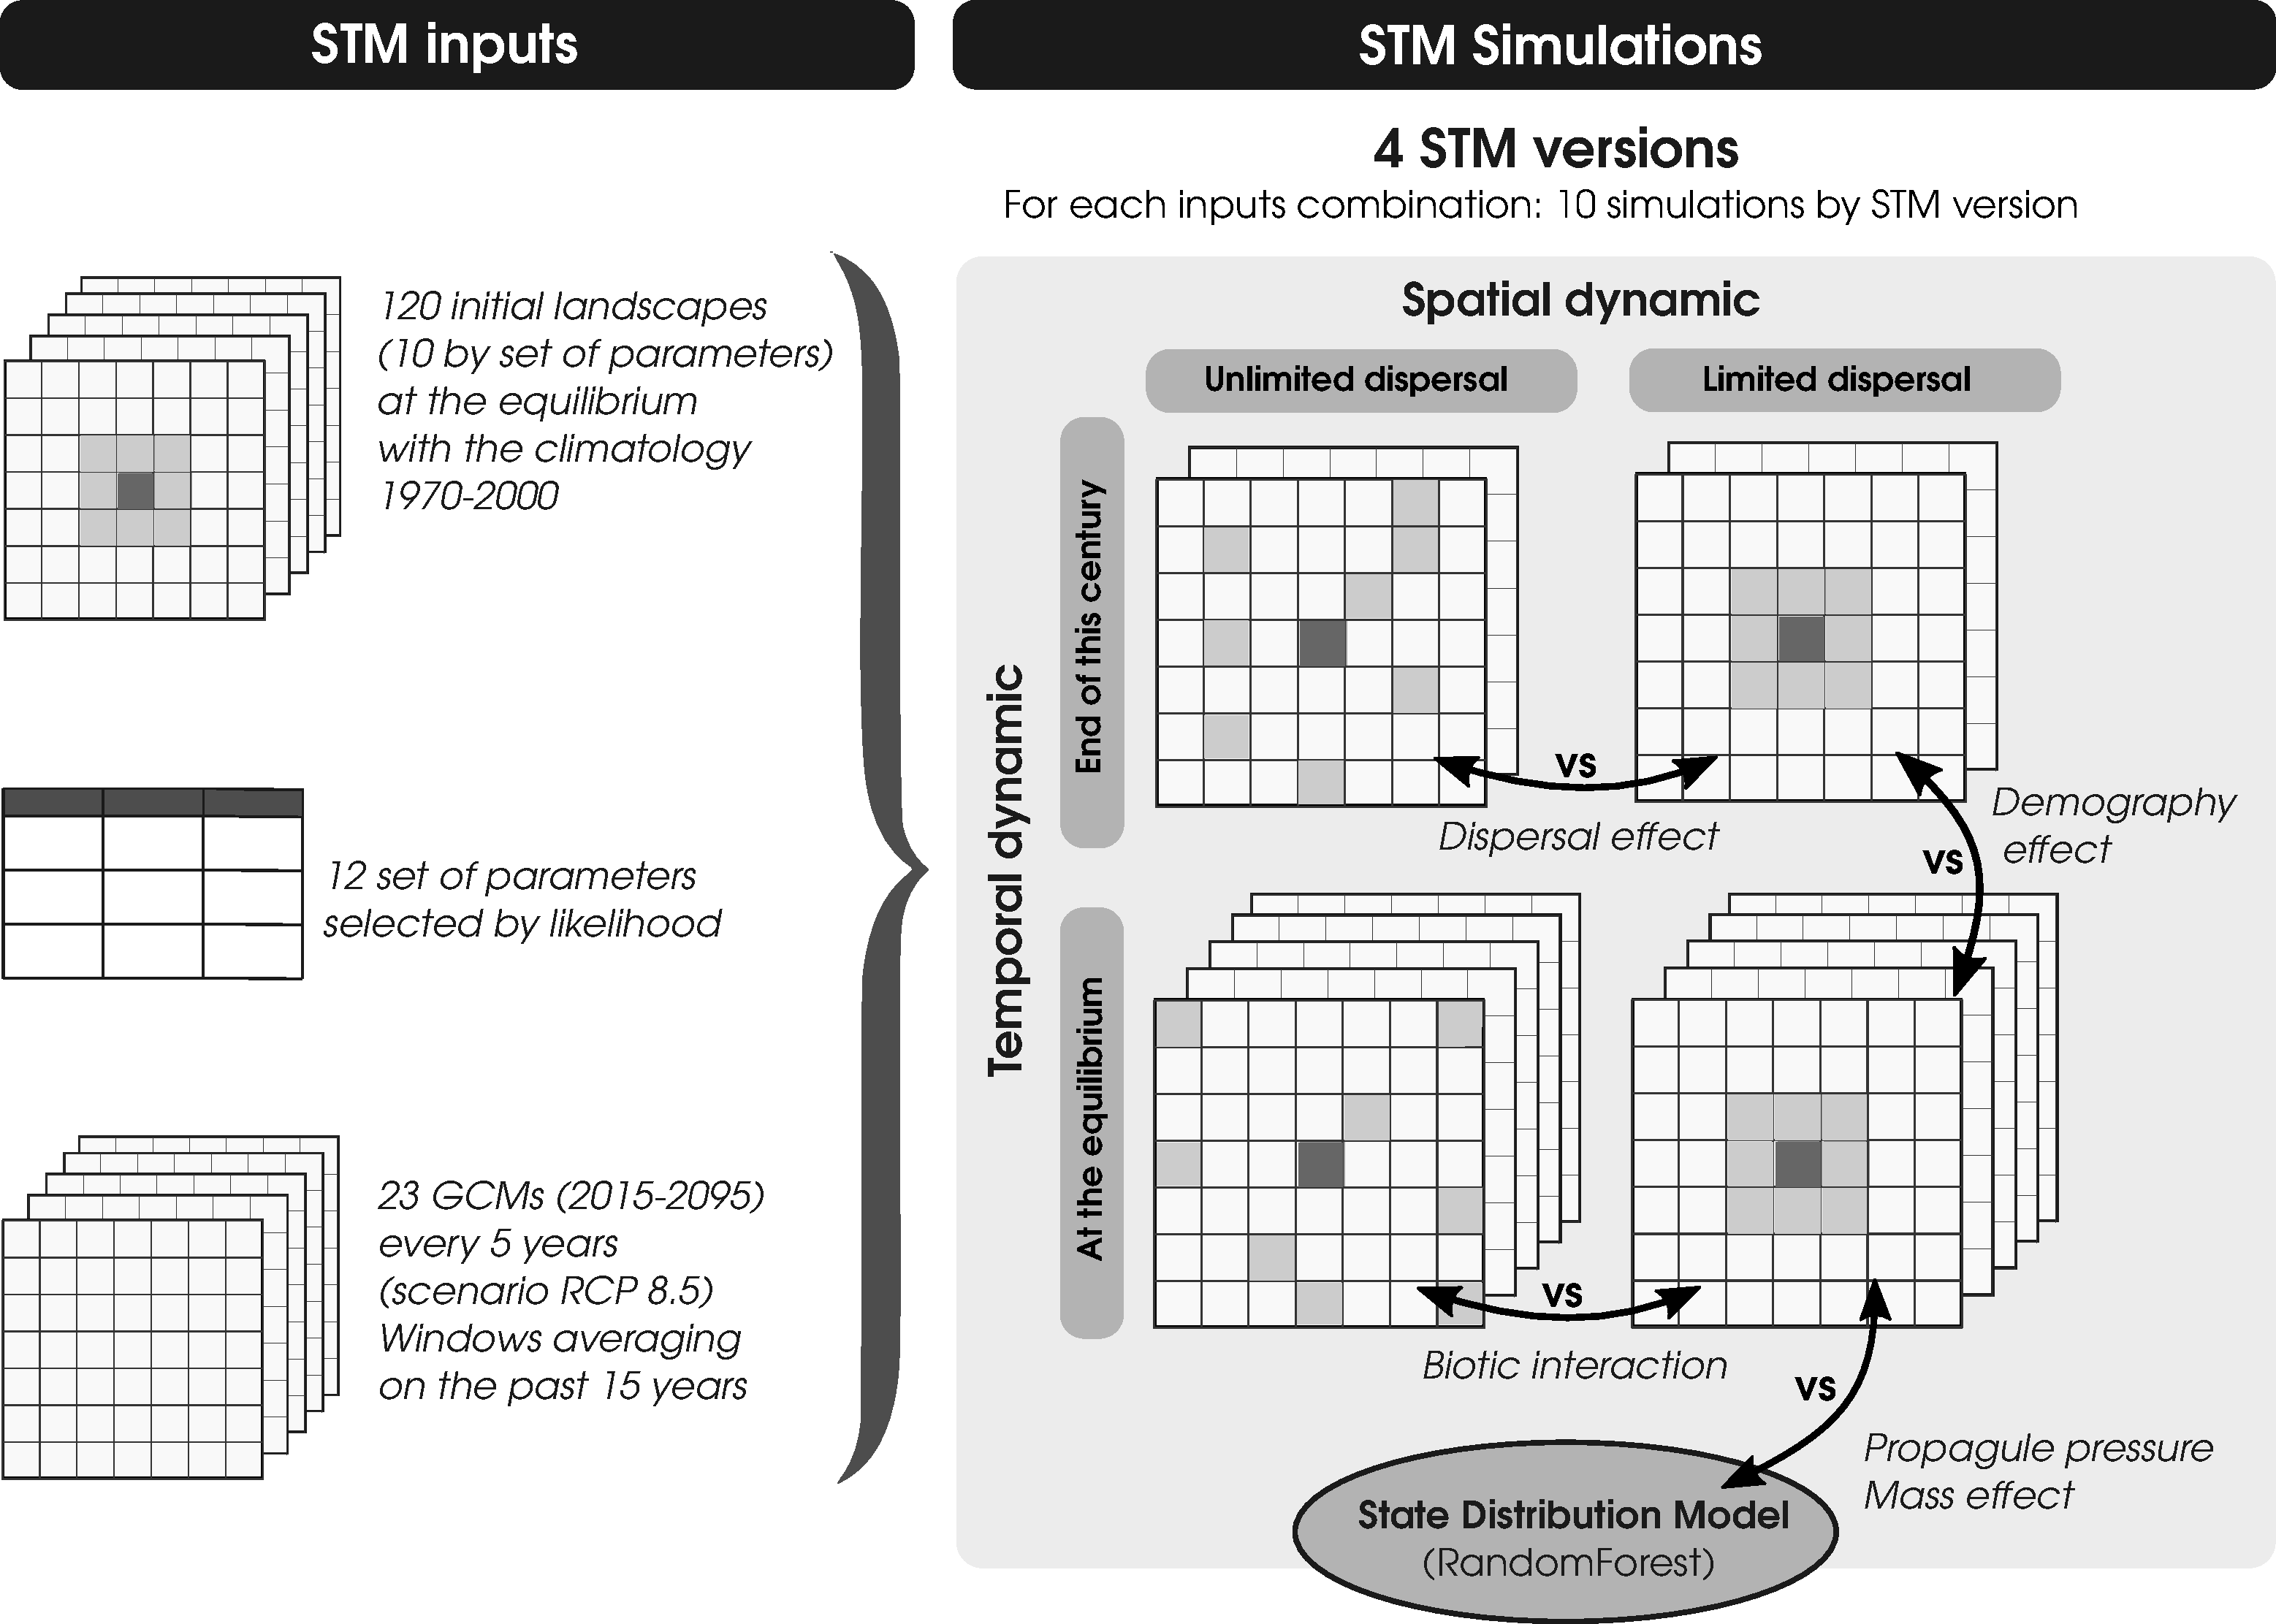
\includegraphics[width=0.9\textwidth]{figs/simus_redu_schema.pdf}
	\end{center}
\end{figure}

% More justification
% Why we choose those climatic variable ? Those climatic variable have been recognized as a good combination to explain the distribution of the boreal forest \cite{Scheffer2012,Goldblum aussi}.

% Mise à l'échelle années pour les transitions


To calibrate the transition probabilities between states based on climate and plot neighbors, we used R (version 3.2.0) and the classification algorithm Random Forest (RandomForest package, version 4.6-10 ) \cite{Liaw2002a}, we incorporated three information types: (1) state transitions observed between plot measurements, (2) the average climate of the 15 years before each measurements for the two climatic variables of interest and finally the (3) the proportion of states available in the neighbors using a SDM (RandomForest) approach as a proxy.

% Ajouter une figure avec le workflow de la calibration

\subsection{Simulations and analysis}

1. How the model is implemented as spatial explicit ? Moore neighbors
Describe the initial simulation landscape and the choice of the resolution


We performed the simulations using 10 several initial landscape, and 12 different sets of parameters. For each parameters set and initial landscape, we ran simulations over the climate predicted by the 23 Global Climate Models (GCM) downscaled at 10 km$^2$ by the Ouranos consortium in clmatology in Quebec. For each of those combinations, we replicated 10 times the simulation in order to take in account the model stochasticty.

\section{Results}

A. Approximation of the neighbors (SDM)
Ajouter la stats du HK pour la validation croisé du modèle.

B. Model simulations

Figure 1. Maps

Facultatif. We found that the STM was able to almost reproduce the actual distribution of the temperate forest and boreal forest.
1. Replacement of mixed forests by temperate forest
2. Long term simulations suggest a further but extremely slow colonization of the temperate forest northward

Figure 2. Boxplot with test

Slow temperate forest demography constrains migration rate more than dispersal limitation. Using the unlimited dispersion version, we predicted that the temperate forest

Spatial interaction prevents the temperate forest to fullfil its predicted niche (SDM) within an ecological timescale.

Complementary analysis on boxplot:
We identified that the STM version explains 90 \% of the latitudinal variance.

The model stochasticity (10 replicates)
The environnemental stochasicity (GCM's; n=23)
Parameters sensitivity (n=12)


New response curve: No leading edge but a higher abondances at the edge. This respond form is uncovered in the \cite{Lenoir2014a} article.


% TODO
%  Complément à apporter dans l'introduction et la conclusion. Importance de l'écologie forestièere vue par Cléments. L'approche par communauté forestière permet de simplifier le travail de conservation.


\clearpage
\bibliography{/home/steve/Dropbox/Bibtex/Master}

\end{document}
